The high-level structure of our proposed metadata package is illustrated in the Figure~\ref{fig:schema_v1} (produced by XMLSpy). 
\begin{figure}
	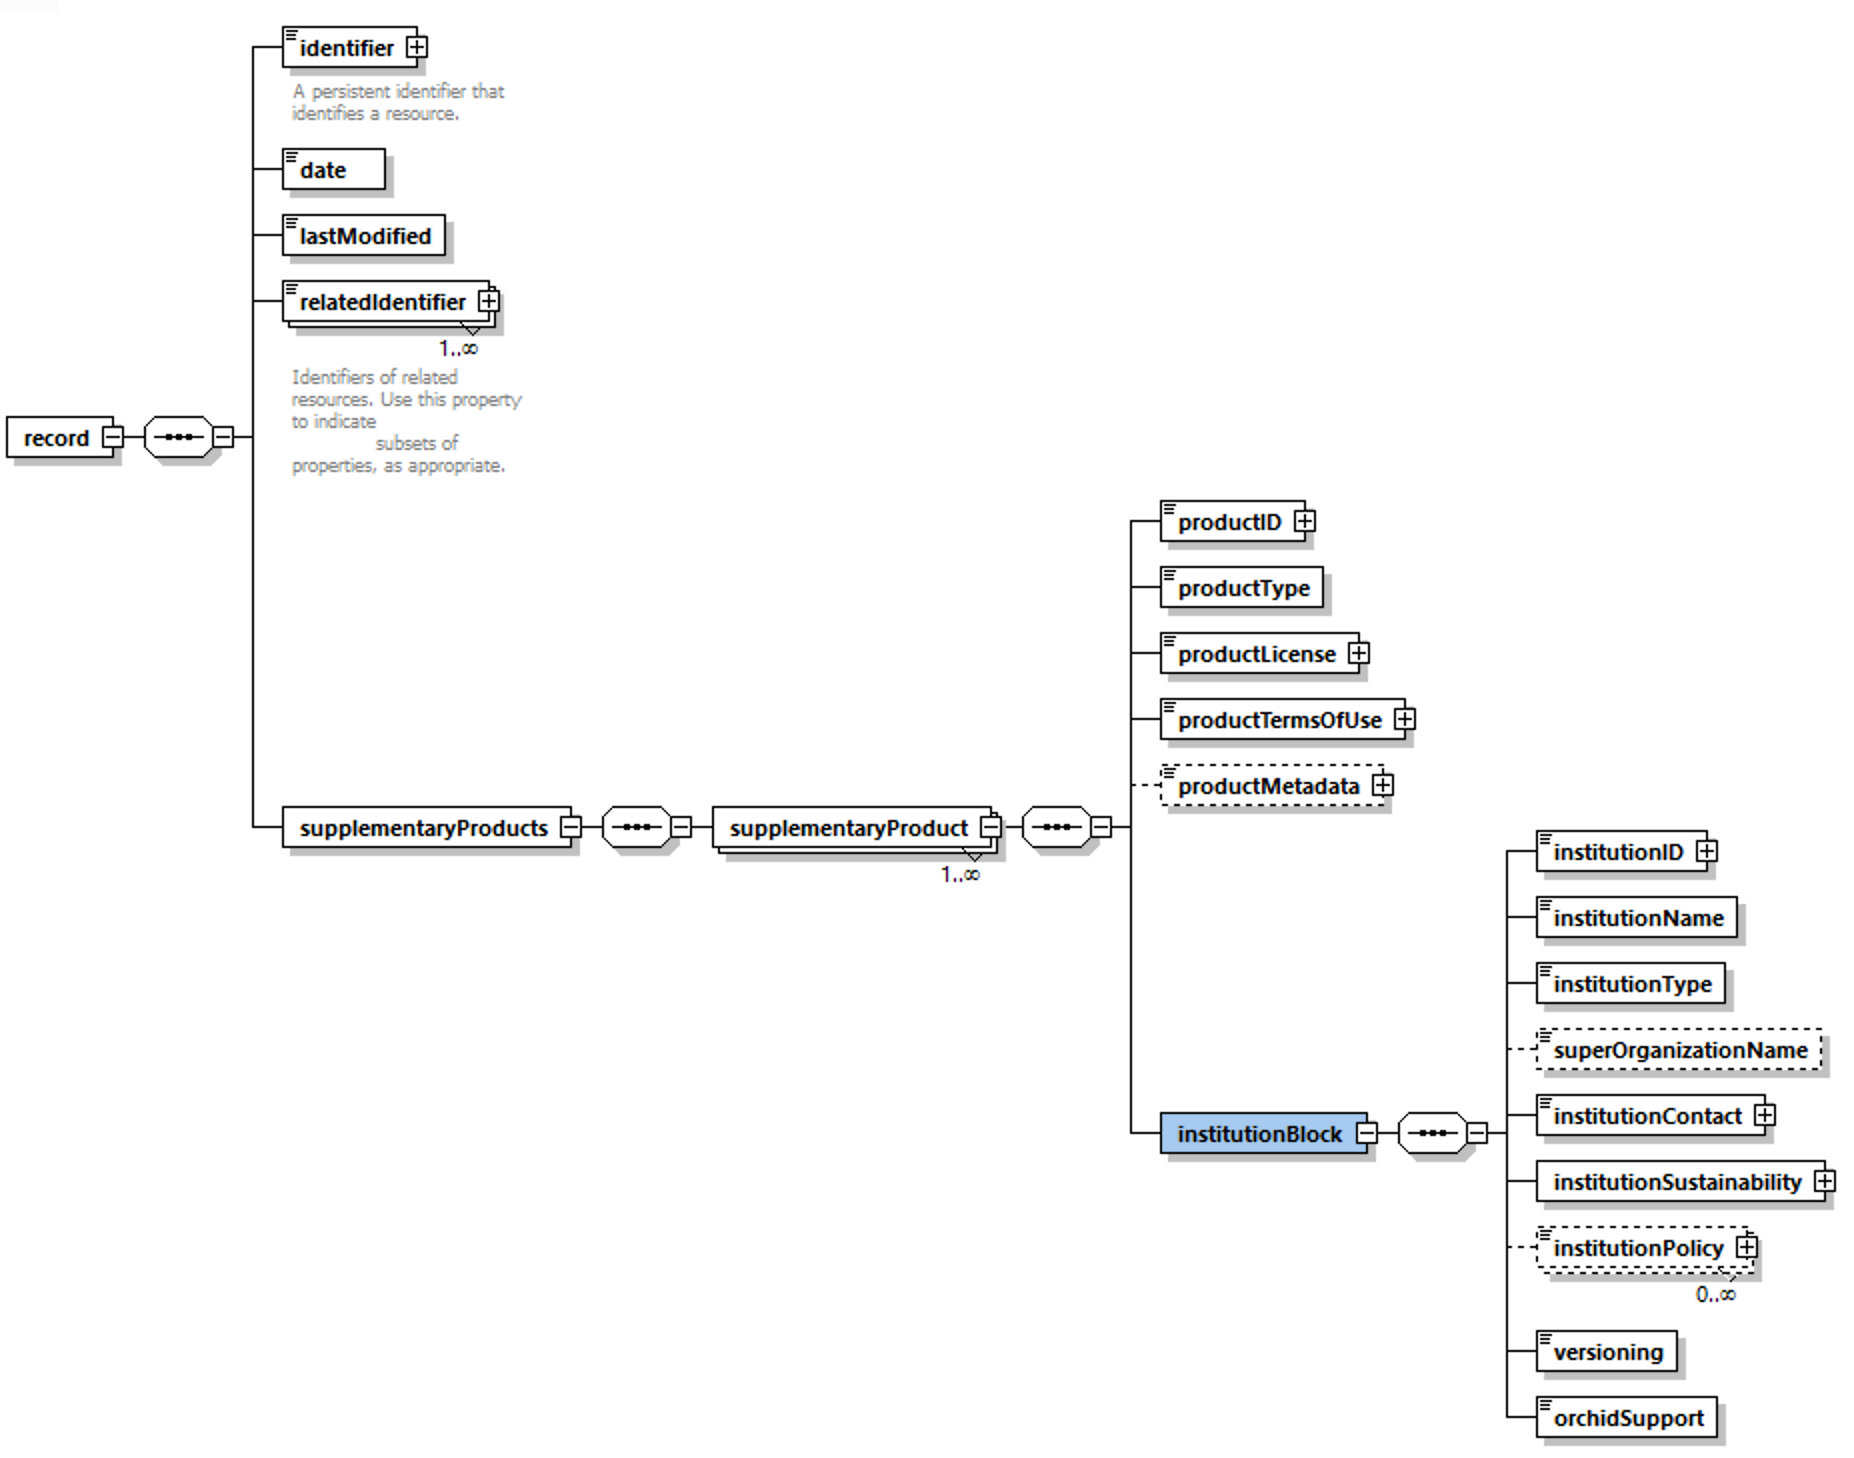
\includegraphics[width=\textwidth]{images/schema_v1}
	\caption{\label{fig:schema_v1}High-level structure of proposed package}
\end{figure} 
As shown, each package is structured as a record, which conceptually models a linkage between a publication and its supplementary materials.  As shown, a record has an identity (DOI), a date created, a last modified date, and the identity (DOI) of the research objects (papers) that are associated with the supplementary products.
Each record then can describe an unlimited number of supplementaryProducts.  Each product has an identifier, a description of its type, licensing information, and linkages to full metadata available elsewhere that fully describes the product.  Finally, each supplementaryProduct has an associated institutionBlock, which contains information about the institutional archive at which the respective supplementaryProduct is located.  
The full annotated schema is available for examination online at (URL TBD).